% BREYI 2026 - Extended Abstract, gaya IEEE (IEEEtran conference).
% Format guidebook tetap dipenuhi: A4, margin atas/bawah 4 cm, kiri/kanan 2 cm,
% Times New Roman 12 pt, spasi tunggal, naskah utama maksimal 5 halaman.
% Kompilasi: xelatex Extended_Abstract_BREYI.tex (2x).
\documentclass[conference,12pt,a4paper]{IEEEtran}
\usepackage[a4paper,top=4cm,bottom=4cm,left=2cm,right=2cm,columnsep=0.6cm]{geometry}
\usepackage{fontspec}
\setmainfont{Times New Roman}[SmallCapsFont={TeX Gyre Termes},SmallCapsFeatures={Letters=SmallCaps}]
\usepackage{amsmath}
\usepackage{unicode-math}
\setmathfont{TeX Gyre Termes Math}
\setmathfont[range={up/{latin,Latin,num}}]{Times New Roman}
\setmathfont[range={it/{latin,Latin}}]{Times New Roman Italic}
\usepackage{graphicx,booktabs,array,tikz,xcolor}
\usetikzlibrary{arrows.meta,positioning,calc,fit}
\usepackage[hidelinks]{hyperref}
\usepackage{xurl}
\urlstyle{same}

\definecolor{ink}{HTML}{262C31}
\definecolor{teal}{HTML}{0F8F84}
\definecolor{tealsoft}{HTML}{E4F2F0}
\definecolor{soft}{HTML}{F2F4F3}

\renewcommand{\figurename}{Gbr.}
\renewcommand{\tablename}{TABEL}
\renewcommand{\abstractname}{Abstrak}
\renewcommand{\IEEEkeywordsname}{Kata kunci}
\renewcommand{\refname}{DAFTAR PUSTAKA}
\newcommand{\eng}[1]{\textit{#1}}
\newcommand{\callout}[3]{\node[circle,fill=teal,text=white,inner sep=0pt,minimum size=12pt,font=\scriptsize\bfseries] at (#1,#2) {#3};}

\begin{document}
\title{Repurposing Second Life EV Batteries for Adaptive Virtual Inertia in Bali's Solar PV Microgrid to Enhance Frequency Stability and Support Renewable Energy Integration}

\author{\IEEEauthorblockN{Mirzariel Akmal Norman, Bagus Aldiguna, Irma Nur Cahyani}
\IEEEauthorblockA{Universitas Gadjah Mada, Yogyakarta, Indonesia\\
Korespondensi: mirzariel@gmail.com}}

\maketitle

\begin{abstract}
Nusa Penida ditargetkan beroperasi dengan 100\% energi terbarukan pada 2030. Ketika porsi PLTS bertambah, jumlah generator diesel yang beroperasi berkurang sehingga inersia sistem turun dan frekuensi jatuh lebih cepat saat terjadi gangguan. Penelitian ini merancang ReVIA, unit \eng{virtual inertia} yang memakai 28 modul baterai kendaraan listrik (EV) bekas. Setiap modul diuji untuk memperoleh \eng{State of Power} (SOP) 10 detik, ditempatkan dalam laci dengan BMS dan konverter DC/DC sendiri, lalu mendapat porsi daya sebanding dengan SOP-nya. Gain inersia ikut diturunkan bila SOP total berkurang. Pada titik desain, ReVIA memberikan 100~kW selama 10~s dengan seluruh modul di bawah 86\% SOP. Pada perangkat yang sama, pembagian daya rata hanya aman sampai 72,7~kW, sedangkan pembagian rata tanpa pembatas memicu trip berantai dalam 0,26~s. Simulasi sistem diesel representatif dengan gangguan 250~kW menunjukkan deviasi nadir frekuensi turun 34\% dan RoCoF turun 36\%, dengan energi hanya 0,156~kWh per kejadian. Estimasi biaya unit adalah Rp509 juta.
\end{abstract}

\begin{IEEEkeywords}
baterai \eng{second-life}, \eng{virtual inertia}, \eng{state of power}, microgrid, Nusa Penida
\end{IEEEkeywords}

\begin{figure*}[!t]
\centering
\begin{minipage}[c]{0.66\textwidth}
\begin{tikzpicture}
\node[anchor=south west,inner sep=0] (img) at (0,0) {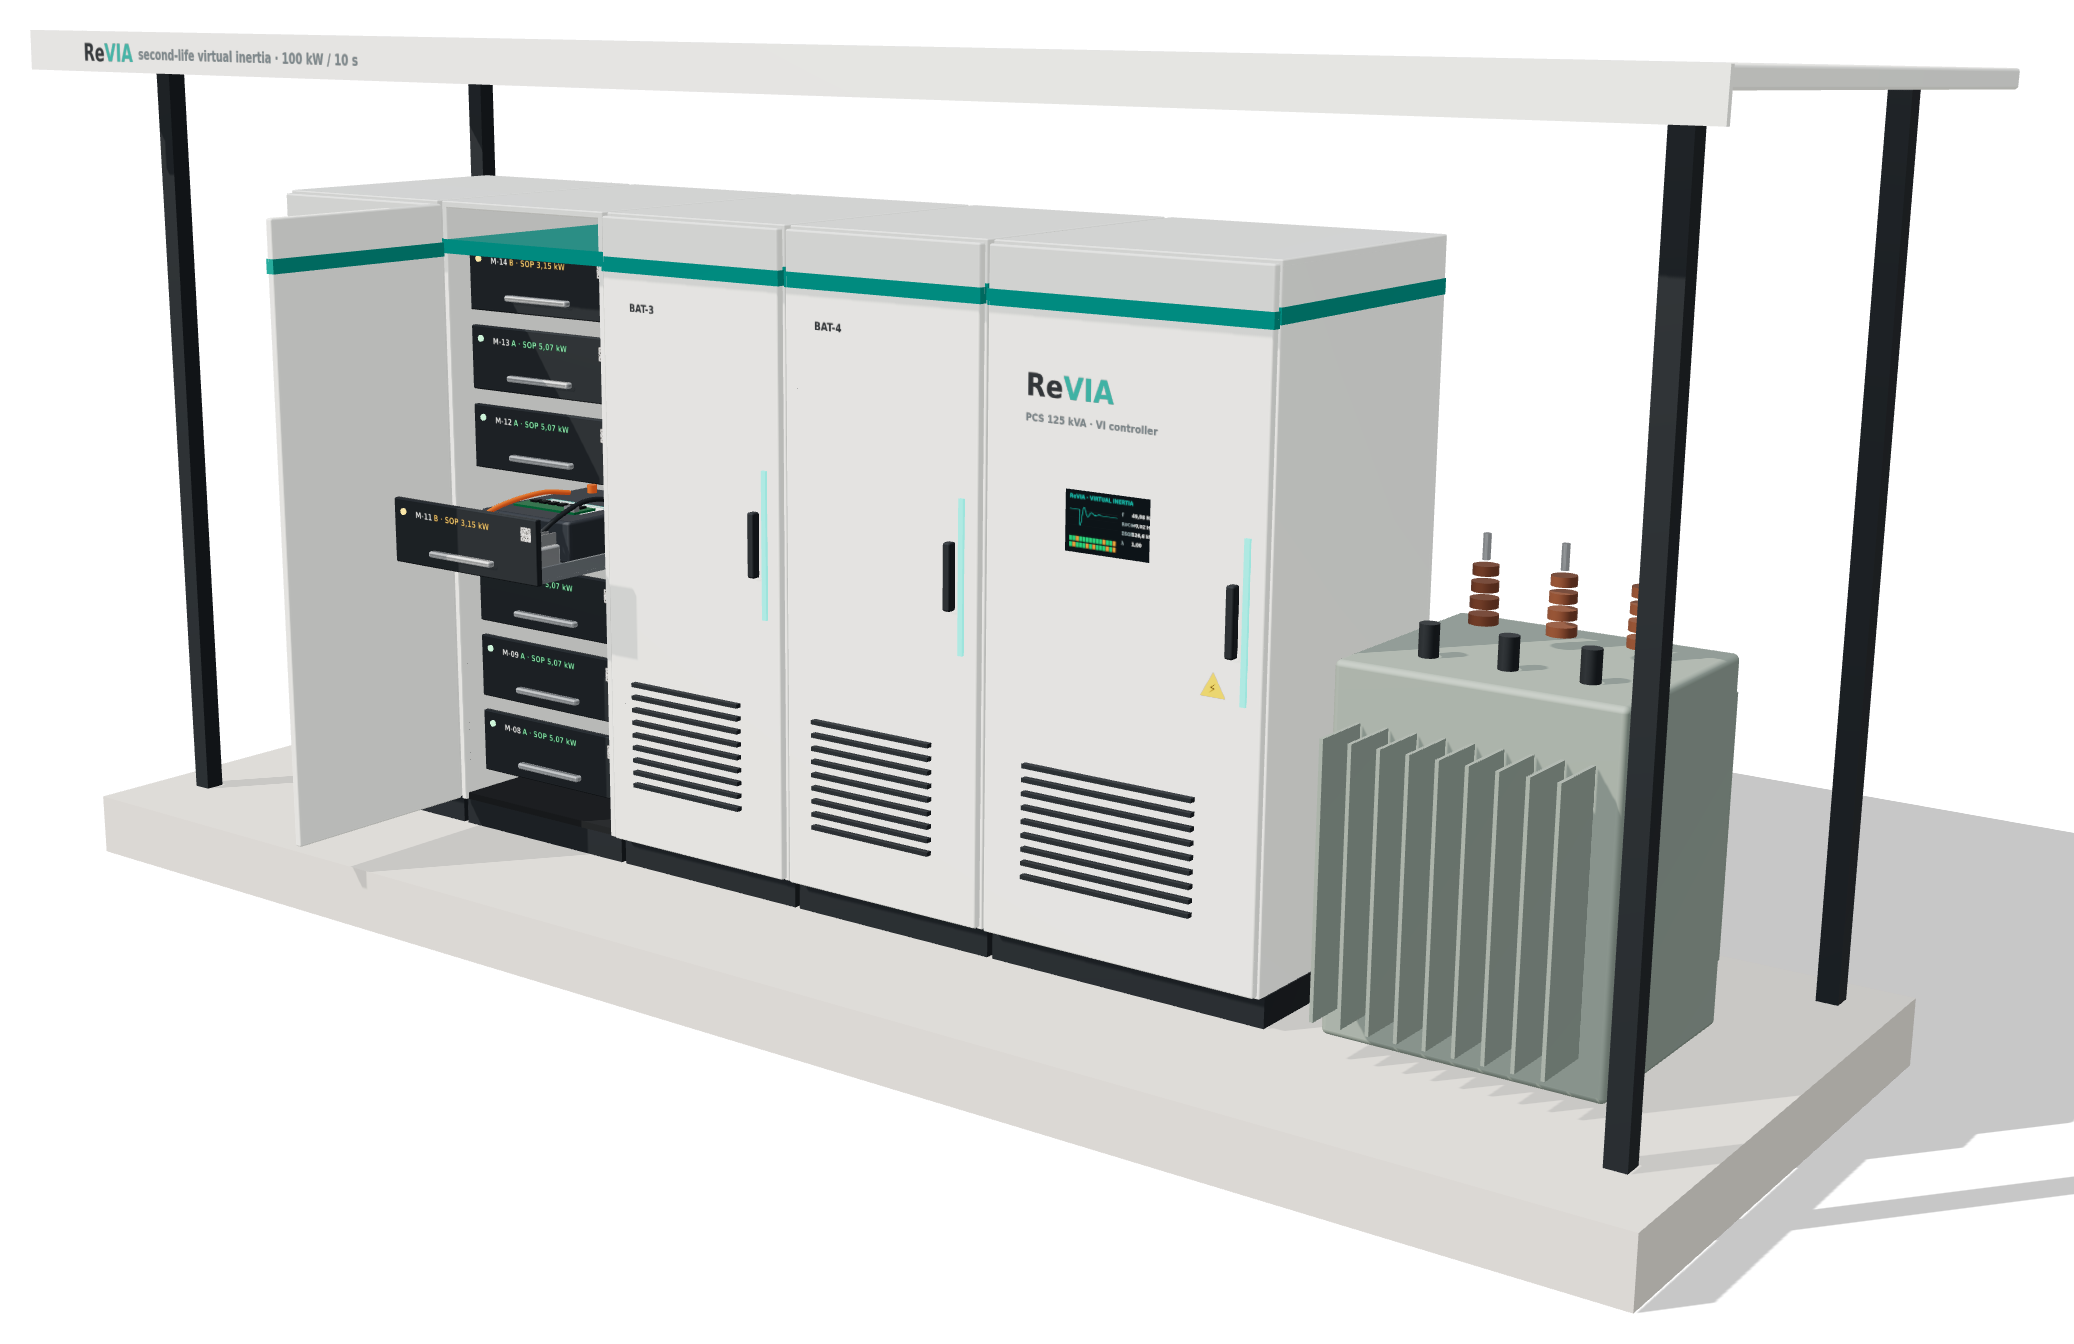
\includegraphics[width=\linewidth]{../figures/render_hero.png}};
\begin{scope}[x={(img.south east)},y={(img.north west)}]
\callout{0.19}{0.70}{1}
\callout{0.37}{0.56}{2}
\callout{0.56}{0.74}{3}
\callout{0.72}{0.50}{4}
\callout{0.16}{0.93}{5}
\end{scope}
\end{tikzpicture}
\end{minipage}\hfill
\begin{minipage}[c]{0.31\textwidth}
\caption{Rancangan 3D ReVIA. (1)~Laci modul yang ditarik untuk penggantian. (2)~Kabinet baterai BAT-1 sampai BAT-4 berisi 28 modul. (3)~Kabinet PCS berisi inverter 125~kVA, pengendali VI, dan layar HMI. (4)~Trafo 0,4/20~kV. (5)~Atap peneduh di atas pad beton.}
\label{fig:render}
\end{minipage}
\end{figure*}

\section{PENDAHULUAN}
\subsection{Latar Belakang}
Pemerintah Provinsi Bali menargetkan Nusa Penida beroperasi dengan 100\% energi terbarukan pada 2030 sebagai bagian dari Bali \eng{Net Zero Emission} 2045 [1], [2]. Sistem kelistrikan pulau ini tercatat sebagai sistem terisolasi [3]. Sejak November 2025, PLN mengoperasikan \eng{smart microgrid} yang menggabungkan PLTS Suana 3,5~MWp, BESS 1,8~MWh, dan PLTD [4].

Pada sistem pulau, energi kinetik rotor generator menjadi penahan pertama perubahan frekuensi. Saat terjadi gangguan daya $\Delta P$, laju perubahan frekuensi awal sebanding dengan $\Delta P/(2HS)$, dengan $H$ konstanta inersia dan $S$ kapasitas generator yang beroperasi [5]. PLTS terhubung melalui inverter dan tidak menyumbang inersia. Jika porsi PLTS naik dan unit diesel yang beroperasi berkurang, nilai $HS$ mengecil. Frekuensi turun lebih cepat dan lebih dalam, pelepasan beban lebih mudah terpicu, dan penambahan PLTS akhirnya dibatasi oleh stabilitas sistem.

\eng{Virtual inertia} (VI) mengatasi masalah ini dengan membuat inverter baterai menyuntikkan daya sebanding laju perubahan frekuensi (RoCoF) selama beberapa detik [6]. Layanan ini membutuhkan daya besar dengan energi kecil. Profil tersebut cocok untuk baterai EV bekas. Kapasitasnya sudah turun ke 70--80\% sehingga kurang layak untuk kendaraan, tetapi modulnya masih sanggup memberi daya pulsa [7], [8].

\subsection{Celah Penelitian dan Kontribusi}
Masalah utama baterai bekas adalah kondisi modul yang tidak seragam. Dua modul dengan kapasitas mirip dapat memiliki resistansi dan batas arus yang jauh berbeda [7], [8]. Jika daya dibagi rata, modul terlemah mencapai batasnya lebih dulu dan seluruh bank harus diturunkan kemampuannya. Liu dkk. [9] membagi daya berdasarkan kapasitas dan SOC pada konverter \eng{cascaded H-bridge} (CHB) 5~kW, tetapi untuk kendali daya aktif-reaktif biasa, belum untuk layanan inersia yang bereaksi dalam orde 100~ms.

Penelitian ini merancang ReVIA (\eng{Repurposed-battery Virtual Inertia, Adaptive}) untuk microgrid Nusa Penida dengan tiga kontribusi:
\begin{enumerate}
\item \textbf{SOP \eng{passport}} per modul. Hasil uji pulsa diringkas menjadi batas daya 10~s yang dicetak sebagai kode QR di laci dan dibaca pengendali.
\item \textbf{Laci modular} berisi BMS dan DC/DC untuk setiap modul, sehingga setiap modul dipakai sampai batasnya sendiri atau dilepas tanpa mematikan unit.
\item \textbf{Kendali VI adaptif} yang membagi daya sebanding SOP dan menurunkan gain inersia saat SOP total berkurang.
\end{enumerate}
Tujuannya adalah menguji kelayakan daya, energi, respons frekuensi, dan biaya rancangan tersebut.

\section{METODOLOGI}
\begin{figure*}[!t]
\centering
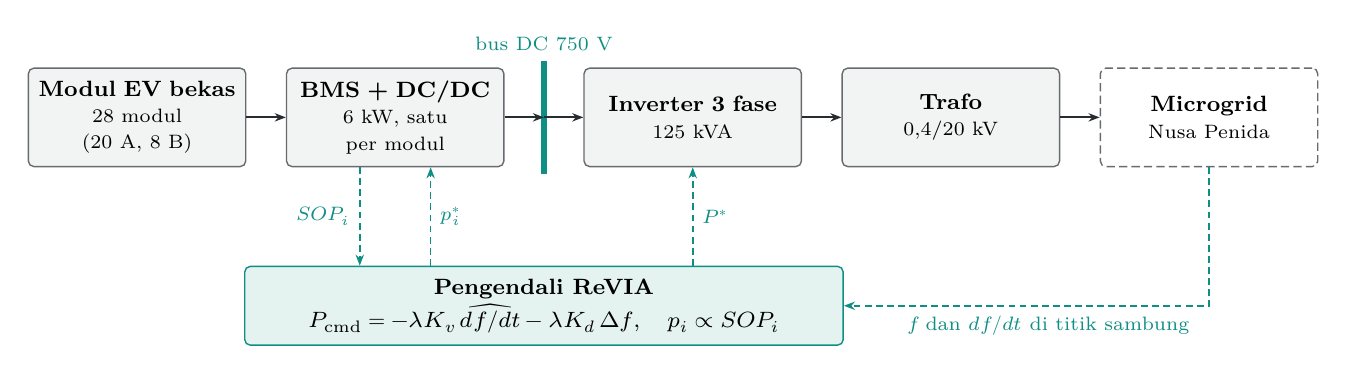
\begin{tikzpicture}[
  font=\footnotesize, >={Stealth[length=4pt]},
  blk/.style={draw=ink!70, line width=0.5pt, rounded corners=2pt, fill=soft, align=center, minimum height=1.25cm, text width=2.55cm, inner sep=3pt},
  pw/.style={->, draw=ink, line width=0.8pt},
  sg/.style={->, draw=teal, line width=0.6pt, dash pattern=on 2.5pt off 1.5pt},
  lbl/.style={font=\scriptsize, text=teal}]
\node[blk] (mod) {\textbf{Modul EV bekas}\\{\scriptsize 28 modul (20 A, 8 B)}};
\node[blk, right=0.5cm of mod] (dc) {\textbf{BMS + DC/DC}\\{\scriptsize 6 kW, satu per modul}};
\coordinate (busx) at ($(dc.east)+(0.5,0)$);
\draw[teal, line width=2.4pt] ($(busx)+(0,0.72)$) -- ($(busx)+(0,-0.72)$);
\node[font=\scriptsize, text=teal, above] at ($(busx)+(0,0.72)$) {bus DC 750 V};
\node[blk, right=1.0cm of dc] (inv) {\textbf{Inverter 3 fase}\\{\scriptsize 125 kVA}};
\node[blk, right=0.5cm of inv] (tr) {\textbf{Trafo}\\{\scriptsize 0,4/20 kV}};
\node[blk, right=0.5cm of tr, fill=white, dash pattern=on 3pt off 1.5pt] (mg) {\textbf{Microgrid}\\{\scriptsize Nusa Penida}};
\draw[pw] (mod) -- (dc);
\draw[pw] (dc.east) -- (busx);
\draw[pw] (busx) -- (inv.west);
\draw[pw] (inv) -- (tr);
\draw[pw] (tr) -- (mg);
\node[draw=teal, fill=tealsoft, line width=0.5pt, rounded corners=2pt, align=center, inner sep=4pt,
      minimum height=1.0cm, minimum width=7.6cm, anchor=north] (ctl)
  at ($(dc.south)!0.5!(inv.south)+(0,-1.25)$)
  {\textbf{Pengendali ReVIA}\\[1pt] $P_{\mathrm{cmd}}=-\lambda K_v\,\widehat{df/dt}-\lambda K_d\,\Delta f,\quad p_i\propto SOP_i$};
\coordinate (s1) at ($(dc.south)+(-0.45,0)$);
\coordinate (s2) at ($(dc.south)+(0.45,0)$);
\draw[sg] (s1) -- node[lbl, left] {$SOP_i$} (s1 |- ctl.north);
\draw[sg] (s2 |- ctl.north) -- node[lbl, right] {$p_i^{*}$} (s2);
\draw[sg] (inv.south |- ctl.north) -- node[lbl, right] {$P^{*}$} (inv.south);
\draw[sg] (mg.south) |- node[lbl, pos=0.72, below] {$f$ dan $df/dt$ di titik sambung} (ctl.east);
\end{tikzpicture}
\caption{Arsitektur ReVIA. Garis tebal menunjukkan aliran daya dan garis putus-putus menunjukkan sinyal kendali.}
\label{fig:arsitektur}
\end{figure*}
\subsection{Lingkup dan Kondisi Acuan}
Kajian dibatasi pada sistem pulau Nusa Penida. Data dinamis sistem, seperti inersia diesel, setelan governor, dan mode kendali BESS eksisting, belum tersedia untuk publik. Karena itu, parameter sistem pada simulasi dinyatakan sebagai asumsi representatif dan dicantumkan lengkap pada Lampiran~A.

\subsection{Seleksi Modul dan SOP Passport}
Setiap modul melewati tahap dokumentasi dan karantina, inspeksi fisik dan isolasi, uji \eng{self-discharge}, uji kapasitas, identifikasi OCV--SOC dan resistansi, serta uji pulsa dua arah pada beberapa SOC dan suhu. Modul cacat ditolak. Dari uji pulsa diperoleh arus maksimum untuk horizon $\tau=10$~s:
\begin{equation}
\begin{aligned}
I_i^{\max}=\min\Big(&I_{\mathrm{OEM}},\ I_{\mathrm{conv}},\ \frac{U_i-V_{\min}}{R_{i,\tau}},\\
&\frac{3600\,Q_i\,(SOC_i-SOC_{\min})}{\tau}\Big)
\end{aligned}
\end{equation}
\begin{equation}
SOP_i=\big(U_i-I_i^{\max}R_{i,\tau}\big)\,I_i^{\max}
\end{equation}
dengan $U_i$ tegangan rangkaian terbuka dan $R_{i,\tau}$ resistansi efektif 10~s. Nilai SOP, resistansi, dan SOH disimpan dalam SOP \eng{passport}. Selama operasi, BMS mengoreksi SOP terhadap SOC dan suhu.

\subsection{Kendali Virtual Inertia Adaptif}
Pengendali mengukur frekuensi $f$ dan RoCoF terfilter di titik sambung. Perintah daya injeksi dan pembagiannya adalah
\begin{equation}
P_{\mathrm{cmd}}=-\lambda K_v\,\widehat{\tfrac{df}{dt}}-\lambda K_d\,(f-f_0)
\end{equation}
\begin{equation}
p_i=P_{\mathrm{t}}\,\frac{SOP_i}{\sum_j SOP_j},\qquad p_i\le\gamma\,SOP_i
\end{equation}
\begin{equation}
\lambda=\min\!\Big(1,\ \frac{\eta\,(\gamma\sum_j SOP_j-P_{\mathrm{aux}})}{P_{\mathrm{svc}}}\Big)
\end{equation}
dengan $P_{\mathrm{t}}$ daya di terminal baterai, $K_v=2H_vS_b/f_0=80$~kW·s/Hz ($H_v=2$~s, $S_b=1$~MW), $K_d=300$~kW/Hz, cadangan ketidakpastian $\gamma=0{,}9$, efisiensi $\eta=0{,}94$, daya bantu $P_{\mathrm{aux}}=2$~kW, dan daya layanan $P_{\mathrm{svc}}=100$~kW. Jika sebuah modul mencapai batas, sisa perintah dialihkan ke modul yang masih memiliki ruang. Proteksi BMS tetap bekerja lokal tanpa menunggu pengendali pusat. Setelah 10~s, layanan diserahkan ke governor diesel dengan \eng{ramp} 5~s. Inverter beroperasi \eng{grid-following}.

\subsection{Evaluasi}
Evaluasi terdiri atas anggaran daya dan energi pada titik desain (OCV 130~V, 25~°C, SOC 50\%) dan simulasi model frekuensi agregat satu area [5] di Python dengan langkah 1~ms. Sistem acuan berupa diesel 3~MVA ($H=1{,}5$~s, droop 5\%), beban 2,5~MW, dan gangguan kehilangan pembangkitan 250~kW. VI dimodelkan dengan filter RoCoF 50~ms dan latensi 100~ms. Semua skema pembagian daya diuji pada perangkat keras yang sama. Pada skema rata tanpa SOP, BMS diasumsikan memutus modul bila arusnya melewati batas lebih dari 50~ms.

\section{HASIL DAN PEMBAHASAN}
\begin{figure*}[!t]
\centering
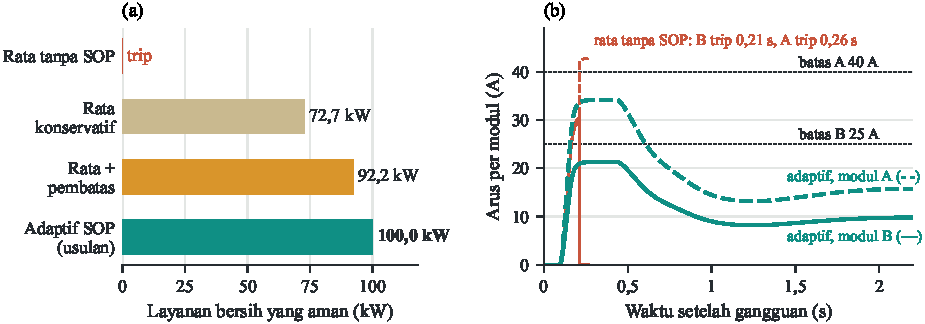
\includegraphics[width=0.92\textwidth]{../figures/fig_alokasi.pdf}
\caption{(a) Layanan bersih yang aman untuk setiap skema pada perangkat keras yang sama. (b) Arus per modul selama gangguan 250~kW. Pembagian rata tanpa SOP memutus modul B lalu modul A, sedangkan ReVIA menjaga semua modul di bawah batasnya.}
\label{fig:alokasi}
\end{figure*}
\subsection{Desain Fisik ReVIA}
ReVIA terdiri atas lima kabinet \eng{outdoor} di atas pad beton (Gbr.~\ref{fig:render}). Empat kabinet baterai masing-masing berisi tujuh laci, sehingga total ada 28 modul NMC/\eng{hard carbon} 36s2p (126~V, 31,5~Ah nominal). Konfigurasi modul mengacu pada sampel EnerDel dalam [8]. Kabinet kelima berisi inverter 125~kVA dan pengendali VI. Trafo 0,4/20~kV menghubungkan unit ke jaringan.

Bentuk kabinet dipilih agar kapasitas dapat ditambah per kabinet dan setiap laci dapat diganti dari depan. Atap peneduh menurunkan beban pendingin di iklim tropis, sedangkan pad beton menjaga peralatan dari genangan di lokasi pesisir. Isi satu laci ditunjukkan pada Gbr.~\ref{fig:laci}. LED panel depan menunjukkan kelas modul, yaitu hijau untuk kelas A dan kuning untuk kelas B. Rancangan mengasumsikan 20 modul kelas A (SOH 80\%, $R_{10\,\mathrm{s}}=0{,}08~\Omega$, batas 40~A) dan 8 modul kelas B (SOH 70\%, 0,16~$\Omega$, 25~A).



\begin{figure}[!t]
\centering
\begin{tikzpicture}
\node[anchor=south west,inner sep=0] (img) at (0,0) {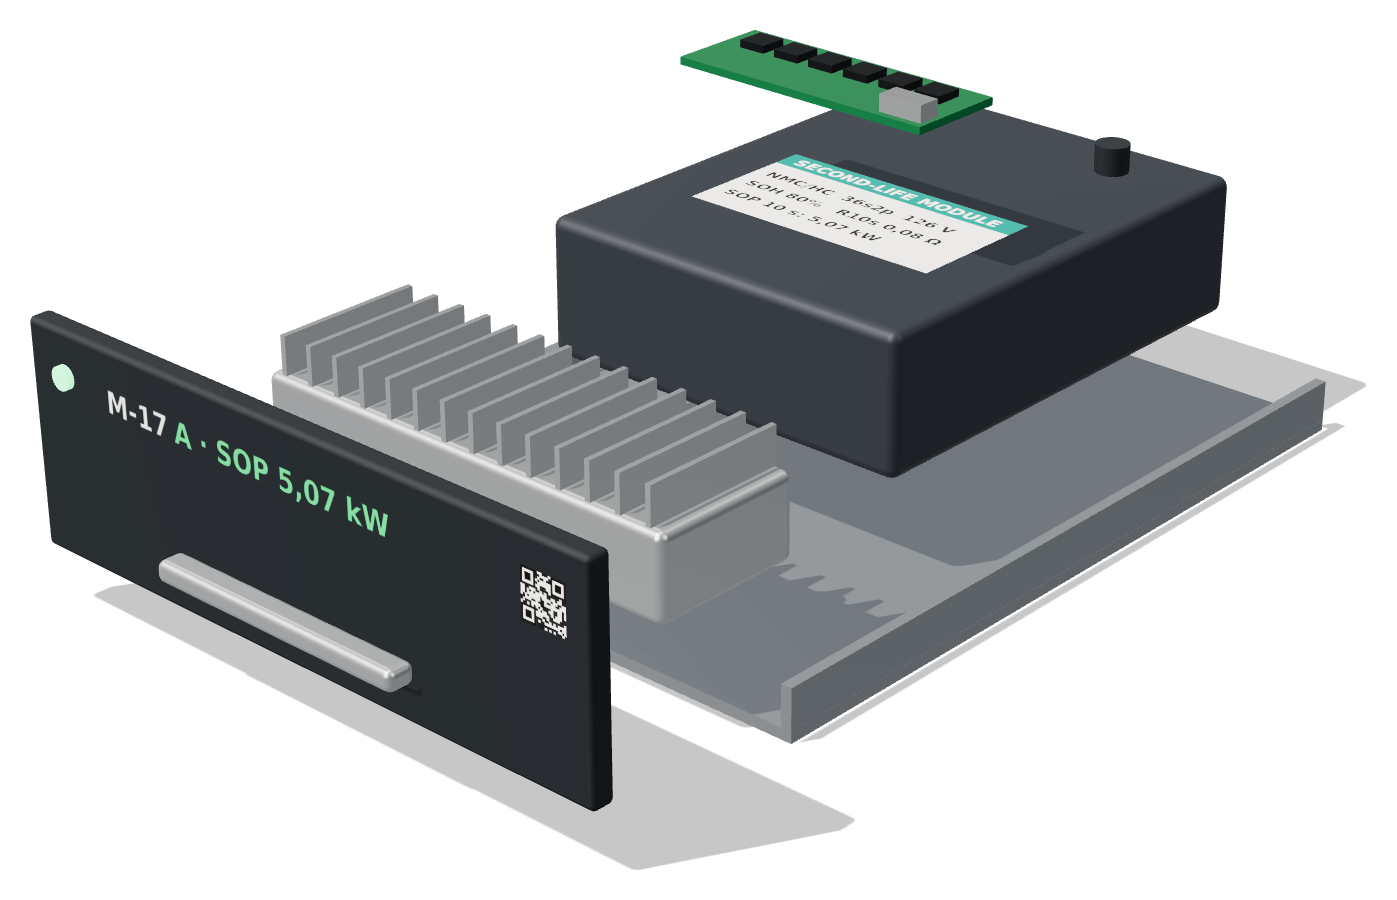
\includegraphics[width=0.92\columnwidth]{../figures/render_drawer.png}};
\begin{scope}[x={(img.south east)},y={(img.north west)}]
\callout{0.86}{0.70}{1}
\callout{0.70}{0.94}{2}
\callout{0.50}{0.62}{3}
\callout{0.06}{0.66}{4}
\callout{0.40}{0.24}{5}
\callout{0.93}{0.45}{6}
\end{scope}
\end{tikzpicture}
\caption{Isi satu laci (\eng{exploded view}): (1) modul EV bekas 126~V, (2) BMS, (3) DC/DC dua arah terisolasi 6~kW, (4) panel depan dengan LED kelas modul, (5) kode QR SOP \eng{passport}, (6) nampan geser.}
\label{fig:laci}
\end{figure}

\subsection{Arsitektur Daya dan Kendali}
Aliran daya dan sinyal ditunjukkan pada Gbr.~\ref{fig:arsitektur}. Setiap modul memiliki DC/DC sendiri menuju bus DC 750~V. Dibanding CHB [9], cara ini membuat arus setiap modul dapat diatur langsung dan modul bermasalah cukup dilepas dari bus. Konsekuensinya adalah 28 konverter senilai Rp84 juta dan tambahan rugi konversi.



\subsection{Anggaran Daya dan Pengaruh Pembagian Daya}
SOP 10~s modul kelas A adalah $(130-40\cdot0{,}08)\cdot40=5{,}07$~kW dan kelas B 3,15~kW, sehingga SOP total 126,64~kW. Dengan cadangan 10\%, daya bantu 2~kW, dan efisiensi 94\%, kemampuan injeksi bersih adalah $0{,}94\,(0{,}9\cdot126{,}64-2)=105{,}26$~kW, di atas kebutuhan 100~kW. Energi per kejadian, termasuk rugi internal dan margin 25\%, hanya 0,40~kWh, sedangkan energi efektif bank 85,7~kWh. Jumlah modul ditentukan oleh kebutuhan daya. Karena itu, baterai bekas yang kapasitas energinya sudah turun tetap layak dipakai.

Pengaruh skema pembagian daya ditunjukkan pada Gbr.~\ref{fig:alokasi}. Pembagian rata membebani setiap modul 3,87~kW, yang bagi modul kelas B berarti arus 30,95~A, di atas batas 25~A. Dalam simulasi, modul B trip pada 0,21~s, bebannya pindah ke modul A, dan modul A ikut trip pada 0,26~s. Seluruh bank lepas di awal kejadian. Pembagian rata yang dibatasi pada kemampuan modul terlemah memang aman, tetapi hanya menghasilkan 72,7~kW. Pembatas lokal tanpa redistribusi menghasilkan 92,2~kW. ReVIA membebani modul A 4,34~kW (34,1~A) dan modul B 2,70~kW (21,3~A), sehingga layanan 100~kW tercapai. Kapasitas ini 37\% lebih besar daripada pembagian rata konservatif.





\subsection{Respons Frekuensi}
Respons frekuensi ditunjukkan pada Gbr.~\ref{fig:frekuensi} dan Tabel~\ref{tab:frek}. Tanpa VI, frekuensi turun ke 49,597~Hz dengan RoCoF $-0{,}803$~Hz/s. Dengan ReVIA, nadir naik ke 49,734~Hz. Deviasi nadir turun dari 0,403~Hz menjadi 0,266~Hz (34\%) dan RoCoF turun 36\%. Energi yang terpakai 0,156~kWh, atau 39\% dari anggaran per kejadian.

Selisih nadir antara ReVIA dan skema rata dengan pembatas lokal hanya 0,008~Hz. Keunggulan ReVIA lebih terlihat pada daya yang dapat dijamin dan pada keamanan modul. Skema rata tanpa SOP sempat membantu sebelum bank trip pada 0,26~s. Setelah itu, sistem berperilaku seperti tanpa VI dan ke-28 modul perlu di-\eng{reset}. Pola yang sama muncul untuk $H=1{,}0$~s (nadir 49,525 menjadi 49,675~Hz) dan $H=2{,}0$~s (49,641 menjadi 49,761~Hz), dan serah-terima ke governor tidak menimbulkan penurunan frekuensi kedua.

\begin{figure}[!t]
\centering
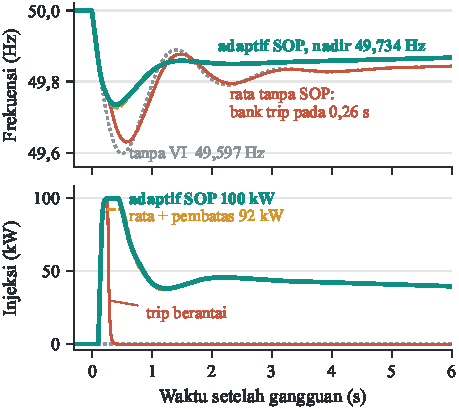
\includegraphics[width=\columnwidth]{../figures/fig_frekuensi.pdf}
\caption{Frekuensi sistem dan daya injeksi VI untuk gangguan 250~kW pada model representatif ($H=1{,}5$~s).}
\label{fig:frekuensi}
\end{figure}

\begin{table}[!t]
\centering
\caption{Metrik Respons Frekuensi (Gangguan 250 kW)}
\label{tab:frek}
\footnotesize
\begin{tabular}{@{}lcccc@{}}
\toprule
Kasus & Nadir & $\Delta$ nadir & RoCoF$^{\dagger}$ & Energi \\
 & (Hz) & turun & (Hz/s) & (kWh) \\
\midrule
Tanpa VI & 49,597 & -- & $-0{,}803$ & -- \\
Rata tanpa SOP & 49,630 & 8\% & $-0{,}722$ & 0,004 \\
Rata konservatif & 49,702 & 26\% & $-0{,}587$ & 0,150 \\
Rata + \eng{clip} & 49,726 & 32\% & $-0{,}532$ & 0,155 \\
\textbf{ReVIA} & \textbf{49,734} & \textbf{34\%} & $\mathbf{-0{,}512}$ & 0,156 \\
\bottomrule
\multicolumn{5}{@{}l}{\scriptsize $^{\dagger}$diukur pada jendela 500 ms setelah gangguan.}
\end{tabular}
\end{table}

\subsection{Biaya, Lingkungan, dan Keterbatasan}
Estimasi biaya ReVIA adalah Rp509,34 juta, termasuk pengujian 35 modul untuk mendapatkan 28 modul layak dan cadangan 15\% (Lampiran~C). Konfigurasi yang sama dengan modul baru diperkirakan Rp568,10 juta. Karena harga masih asumsi, perbandingan akhir akan memakai \eng{net present cost} dan LCA untuk layanan setara 100~kW/10~s.

Keterbatasan rancangan ini adalah parameter dinamis Nusa Penida yang belum diperoleh dari PLN, parameter modul yang masih berupa kriteria penerimaan, dan model agregat yang belum menangkap dinamika PLL serta bus DC. Opsi pembaruan kendali BESS eksisting juga perlu dibandingkan.

\section{KESIMPULAN}
ReVIA mengubah 28 modul baterai EV bekas yang tidak seragam menjadi layanan \eng{virtual inertia} 100~kW/10~s untuk microgrid Nusa Penida melalui SOP \eng{passport}, laci dengan DC/DC sendiri, dan pembagian daya sebanding SOP. Dengan baterai yang sama, daya aman naik 37\% dibanding pembagian rata konservatif dan trip berantai dapat dicegah. Pada model representatif, deviasi nadir turun 34\% dan RoCoF turun 36\% dengan energi 0,156~kWh per kejadian. Tahap berikutnya adalah validasi dengan data PLN dan modul nyata, lalu uji \eng{hardware-in-the-loop}.

\begin{thebibliography}{99}
\footnotesize
\bibitem{b1} Dinas Ketenagakerjaan dan ESDM Provinsi Bali, ``Menghadiri rapat progres implementasi peta jalan Nusa Penida 100\% energi terbarukan,'' 27 Apr. 2026. [Daring]. Tersedia: \url{https://disnakeresdm.baliprov.go.id/menghadiri-rapat-progres-implementasi-peta-jalan-nusa-penida-100-energi-terbarukan/}
\bibitem{b2} BRIDA Provinsi Bali, ``Kunjungan ke lokasi PLTD di Desa Kutampi dan PLTS Hybrid di Desa Suana Nusa Penida,'' 17 Jul. 2025. [Daring]. Tersedia: \url{https://brida.baliprov.go.id/kunjungan-ke-lokasi-pembangkit-listrik-tenaga-diesel-pltd-di-desa-kutampi-dan-pembangkit-listrik-tenaga-surya-plts-hybrid-di-desa-suana-nusa-penida}
\bibitem{b3} Ditjen Ketenagalistrikan, Kementerian ESDM, \textit{Laporan Kinerja Ditjen Ketenagalistrikan Tahun 2024}. [Daring]. Tersedia: \url{https://www.esdm.go.id/assets/media/content/content-laporan-kinerja-ditjen-ketenagalistrikan-tahun-2024.pdf}
\bibitem{b4} PT PLN (Persero), ``PLN operasikan smart microgrid berbasis energi hijau di Nusa Penida Bali,'' Siaran Pers No. 241.PR/STH.01.05/XI/2025, 13 Nov. 2025. [Daring]. Tersedia: \url{https://web.pln.co.id/media/siaran-pers/2025/11/pln-operasikan-smart-microgrid-berbasis-energi-hijau-di-nusa-penida-bali}
\bibitem{b5} P. Kundur, \textit{Power System Stability and Control}. New York, NY, USA: McGraw-Hill, 1994.
\bibitem{b6} U. Tamrakar, D. Shrestha, M. Maharjan, B. P. Bhattarai, T. M. Hansen, and R. Tonkoski, ``Virtual inertia: Current trends and future directions,'' \textit{Appl. Sci.}, vol. 7, no. 7, Art. no. 654, 2017, doi: 10.3390/app7070654.
\bibitem{b7} A. Hassan \textit{et al.}, ``Second-life batteries: A review on power grid applications, degradation mechanisms, and power electronics interface architectures,'' \textit{Batteries}, vol. 9, no. 12, Art. no. 571, 2023, doi: 10.3390/batteries9120571.
\bibitem{b8} C. White, B. Thompson, and L. G. Swan, ``Repurposed electric vehicle battery performance in second-life electricity grid frequency regulation service,'' \textit{J. Energy Storage}, vol. 28, Art. no. 101278, 2020, doi: 10.1016/j.est.2020.101278.
\bibitem{b9} C. Liu, X. Cai, and Q. Chen, ``Self-adaptation control of second-life battery energy storage system based on cascaded H-bridge converter,'' \textit{IEEE J. Emerg. Sel. Topics Power Electron.}, early access, 2018, doi: 10.1109/JESTPE.2018.2886965.
\bibitem{b10} M. Rasheed \textit{et al.}, ``Active reconditioning of retired lithium-ion battery packs from electric vehicles for second-life applications,'' \textit{IEEE J. Emerg. Sel. Topics Power Electron.}, vol. 12, no. 1, pp. 388--404, 2024, doi: 10.1109/JESTPE.2023.3325251.
\end{thebibliography}

\clearpage
\onecolumn
\section*{Lampiran}
\small
\noindent\textbf{A. Parameter Rancangan dan Simulasi}\\[3pt]
\begin{tabular}{@{}p{6.4cm}p{4.6cm}p{5.6cm}@{}}
\toprule
Parameter & Nilai & Status \\
\midrule
Kimia dan konfigurasi modul & NMC/HC, 36s2p & Acuan sampel EnerDel [8] \\
Tegangan rerata; kapasitas nominal & 126 V; 31,5 Ah & Data acuan [8] \\
Jumlah modul aktif & 20 kelas A + 8 kelas B & Asumsi (35 diuji, 80\% lolos) \\
Kapasitas efektif A/B & 25,2 / 22,05 Ah & Asumsi SOH 80\% / 70\% \\
OCV titik hitung; $R_{10\,\mathrm{s}}$ A/B & 130 V; 0,08 / 0,16 $\Omega$ & Asumsi, diganti hasil uji \\
Batas arus pengosongan A/B & 40 / 25 A & Kriteria penerimaan \\
Jendela SOC; suhu titik hitung & 30--70\% (awal 50\%); 25 °C & Asumsi operasi \\
DC/DC per modul; bus DC; inverter & 6 kW; 750 V; 125 kVA & Asumsi arsitektur \\
Efisiensi satu arah; daya bantu & 94\%; 2 kW & Asumsi, perlu diukur \\
$K_v$; $K_d$; $\gamma$ & 80 kW·s/Hz; 300 kW/Hz; 0,9 & Parameter desain \\
Filter RoCoF; latensi; loop arus inverter & 50 ms; 100 ms; 20 ms & Target uji \\
Diesel; $H$; droop; lag governor--mesin & 3 MVA; 1,5 s; 5\%; 0,5 s & Representatif, bukan data PLN \\
Beban; redaman beban; kendali sekunder & 2,5 MW; 1 pu; 0,05 MW/(Hz·s) & Representatif \\
Penundaan trip BMS (skema rata) & 50 ms & Asumsi \\
\bottomrule
\end{tabular}

\vspace{8pt}
\noindent\textbf{B. Perhitungan Daya, Arus, dan Energi}\\[2pt]
$V_A=130-40(0{,}08)=126{,}8$ V, $SOP_A=5{,}072$ kW; $V_B=130-25(0{,}16)=126{,}0$ V, $SOP_B=3{,}150$ kW; $\sum SOP=20(5{,}072)+8(3{,}150)=126{,}64$ kW. Kemampuan bersih $0{,}94[0{,}9(126{,}64)-2]=105{,}26$ kW. Kebutuhan terminal untuk 100 kW bersih adalah $100/0{,}94+2=108{,}38$ kW dengan faktor pembagian $108{,}38/126{,}64=0{,}856$. Alokasi ReVIA: $p_A=4{,}341$ kW, $p_B=2{,}696$ kW. Arus dihitung dengan $I=\big(U-\sqrt{U^2-4RP}\big)/(2R)$, sehingga $I_A=34{,}11$ A dan $I_B=21{,}30$ A. Pembagian rata: $108{,}38/28=3{,}871$ kW per modul dan $I_B=30{,}95$ A. Setelah modul B lepas, $108{,}38/20=5{,}42$ kW per modul A dan $I_A=42{,}8$ A $>$ 40 A. Rata + clip: $0{,}94[20(3{,}871)+8(2{,}835)-2]=92{,}21$ kW. Rata konservatif: $0{,}94[28(0{,}9)(3{,}15)-2]=72{,}74$ kW. Energi AC per kejadian $100\cdot10/3600=0{,}278$ kWh. Energi di sisi terminal 0,301 kWh. Rugi internal $20I_A^2R_A+8I_B^2R_B=2{,}44$ kW selama 10 s menambah 0,0068 kWh. Dengan margin 25\%, totalnya $0{,}385\approx0{,}40$ kWh. Energi efektif bank adalah $126[20(25{,}2)+8(22{,}05)]/1000=85{,}73$ kWh. Jika satu modul A dilepas, kemampuan bersih masih 100,97 kW.

\vspace{8pt}
\noindent\textbf{C. Rencana Anggaran Biaya (juta rupiah, asumsi 2026)}\\[3pt]
\begin{tabular}{@{}p{8.2cm}p{5.6cm}r@{}}
\toprule
Komponen & Basis & Biaya \\
\midrule
Pengadaan modul bekas & 35 × Rp1,50 juta & 52,50 \\
Pengujian dan karakterisasi & 35 × Rp0,40 juta & 14,00 \\
Repurposing mekanik, BMS, dan sensor & 28 × Rp0,75 juta & 21,00 \\
DC/DC terisolasi dua arah & 28 × Rp3,00 juta & 84,00 \\
Inverter 125 kVA dan trafo antarmuka & 1 + 1 unit & 125,00 \\
Proteksi DC/AC dan monitoring isolasi & paket & 40,00 \\
Kabinet, pendingin, proteksi kebakaran & paket & 50,00 \\
Kendali, \eng{engineering}, \eng{commissioning}, logistik & paket & 55,00 \\
Penanganan 7 modul yang ditolak & 7 × Rp0,20 juta & 1,40 \\
\midrule
Subtotal / cadangan 15\% & & 442,90 / 66,44 \\
\textbf{Total} & & \textbf{509,34} \\
\bottomrule
\end{tabular}\\[3pt]
Pembanding dengan modul baru (28 × Rp4 juta, tanpa modul ditolak, komponen lain sama) adalah Rp568,10 juta. Semua harga merupakan asumsi dan bukan penawaran vendor.

\vspace{8pt}
\noindent\textbf{D. Posisi Kebaruan dan Peta Jalan}\\[3pt]
\begin{tabular}{@{}p{3.3cm}p{6.3cm}p{7.0cm}@{}}
\toprule
Unsur & Sudah ada dalam literatur & Yang ditambahkan ReVIA \\
\midrule
Baterai EV bekas & Seleksi, degradasi, BMS [7], [8]; rekondisi [10] & Hasil uji langsung menjadi batas daya layanan (SOP \eng{passport}) \\
Pembagian daya adaptif & Berbasis kapasitas dan SOC pada CHB 5 kW [9] & Berbasis SOP 10 s untuk layanan cepat, dengan redistribusi \\
\eng{Virtual inertia} & Konsep kendali yang sudah mapan [6] & Gain inersia $\lambda K_v$ mengikuti kemampuan nyata bank bekas \\
Konteks Bali & Target Nusa Penida 100\% EBT [1], [4] & Unit tambahan modular dengan pembanding yang jelas \\
\bottomrule
\end{tabular}\\[4pt]
Peta jalan: (1) data dinamis dan perbandingan dengan pembaruan kendali BESS eksisting bersama PLN; (2) pengadaan dan karakterisasi modul nyata; (3) kalibrasi model SOP dan simulasi EMT; (4) uji \eng{hardware-in-the-loop} skema rata dan ReVIA; (5) demonstrasi terbatas di bawah pengawasan operator. Kode simulasi tersedia di repositori tim.

\end{document}
